\subsection{\F{OLYMPUS}}\label{sec:olympus}

UKAEA has a history dating back to the 1960s of pioneering software engineering
techniques, particularly for nuclear fusion applications. K.V.~Roberts promoted
what is now known as ``literate programming"~\cite{Ro69Publ} and subsequently
introduced the \F{OLYMPUS} programming system~\cite{Ch74Stan} which includes design patterns
and modules (that could contain more than one subroutine) that constitute a framework within the definition
of Sommerville as discussed in \Sec{intro}. \F{OLYMPUS} is further described
in the textbook by Hockney and Eastwood~\cite[\S\,3]{hockneyeastwood}.

The main \F{OLYMPUS} design pattern is of enduring interest, especially now that
HPC architectures place a premium on managing memory. The assumption is that
at heart all physics software has one outermost loop, corresponding either
to iterating
to a converged solution of the model or to representing system evolution in time, and that
convergence or elapse of sufficient physical time may not have occurred
when the loop terminates. For efficient use of machine resources, it is 
desirable that the computation restarts from where it terminated, 
minimising the amount of information to be stored between calculations.
\F{OLYMPUS} also allowed for parameters to change at restart, an
issue which still might arise nowadays when tracking bifurcations of solutions of
nonlinear models.

The design pattern illustrated in \Fig{cronos} handles the restart problem
which as indicated has the potential to become tricky, as common routines to read
control data ({\tt DATA}) and calculate derived constants~({\tt AUXVAL}) have
to be interspersed with others which only need be called at the
start of the first calculation~({\tt PRESET}) or at restart~({\tt RESUME}).
Thus using the framework eliminates the need for a certain amount of thought,
and perhaps more helpfully, a good deal of documentation, since a standard
reference can be quoted.
\begin{figure}
\centerline{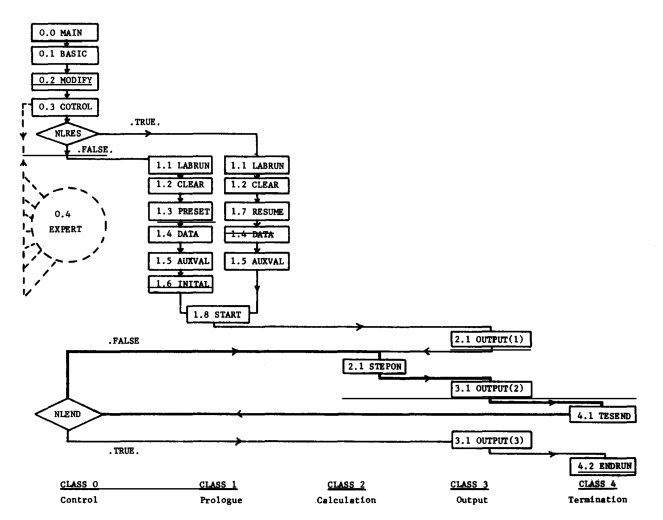
\includegraphics[width=0.9\textwidth]{../pics/cronos}}
\caption{Fig.~1 from ref~\protect\cite{Ch74Stan}, showing
the top-level design pattern. The thick line indicates
the main loop.\label{fig:cronos}}
\end{figure}

\Fig{olympus_diagn} shows a second pattern built around the \F{OLYMPUS}
library of modules such as {\tt MESAGE} and~{\tt HVAR}.
The library is of no intrinsic interest now because it is mostly
concerned with either timing or string handling. Nonetheless it is important
as an early example of `separation of concerns' to provide portability
between machines.  In the 1970s the local computing service
might well have had to implement the \F{OLYMPUS} library in machine-specific
assembly code.  Nowadays, computer languages have as standard very flexible
timing and string handling functions, that emerged out of a set of largely
ad hoc libraries like \F{OLYMPUS}.  Hopefully a similar upgrade path will 
ultimately be followed by HPC coding of for example array-based manipulations
that currently can only be implemented efficiently in an architecture-dependent way.

\begin{figure}
\centerline{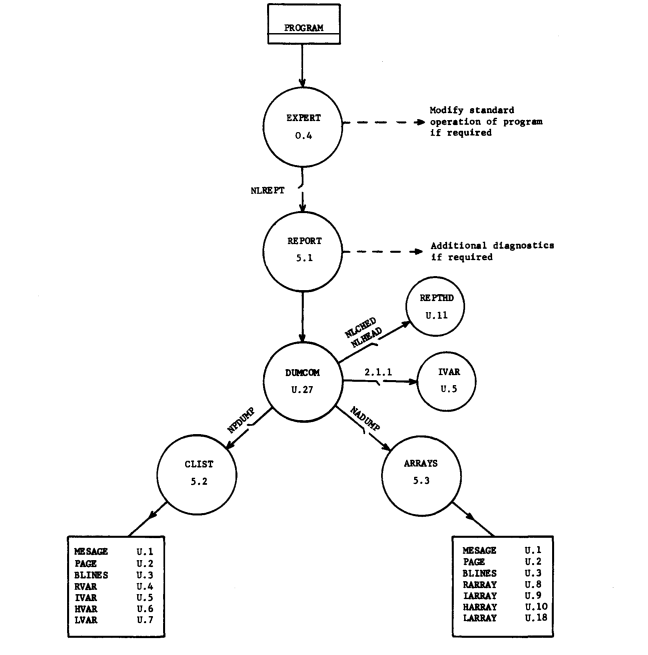
\includegraphics[width=0.9\textwidth]{../pics/olympus_diagn}}
\caption{Fig.~4 from ref~\protect\cite{Ch74Stan}, showing the
diagnostic design pattern, and indicating library routines
(with the ``U"~classification).\label{fig:olympus_diagn}}
\end{figure}

\subsection{\F{SMARDDA} Modules}\label{sec:smardda}
The U(nix)-\F{OLYMPUS} tools were developed from \F{OLYMPUS} in the late 1980s with the recognition that Unix$^{TM}$
was becoming the default operating system for scientific work. They represented a 
combination of the \F{OLYMPUS} framework above and C~shell scripts designed to enhance programmer
productivity, both at the individual level, by eg.\ 
accepting free format input of FORTRAN code and documentation, and at team level
by promoting use of standard data and calling structures, and indeed workflows.
The new Fortran standards emerging in the 1990s as Fortran~90 and Fortran~95 reduced
the need for many of the U-\F{OLYMPUS} features, Linux largely replaced Unix, and U-\F{OLYMPUS}
was not further updated. For Fortran~95 developments, emphasis switched
more on to promoting a coherent style, to exploit the object-oriented features
of the Fortran~95 language efficiently.  This style was eventually published in ref~\cite{fprog},
which includes templates for typical object complexities.

\paragraph{Physics and Scope}
The \F{SMARDDA} modules~\cite{Wa14b} are a 21st Century development of object-oriented software
in this style for magnetic fusion applications.  The \F{SMARDDA} modules
were originally developed for neutronics~\cite{Wa09a} and neutral beam duct design~\cite{Wa15}.
As a result of the latter, the basic \F{SMARDDA} algorithm was designed to be efficient both for
short ``rays" representing gyro-orbit segments as well as ``long rays" representing
neutrals and neutron paths, by combining two pre-existing algorithms, SMART and DDA.
Ionised particle trajectories in the ducts were treated using the well-known Boris
algorithm~\cite[\S\,4-7]{hockneyeastwood}.
In the subsequent development for fieldline tracing~\cite{Wa14b}, the fact that the magnetic field was likely to 
be a solution of the discretised Grad-Shafranov equation that was only second order accurate in mesh-spacing led to the 
implementation of a low order Runge-Kutta integration scheme for following the field. An adaptive
(Fehlberg or Embedded method RKF23) time-stepping scheme was used purely to avoid the problem of
selecting an initial time-step. Hence through a sequence of different applications,
software was developed capable of following over $100$~million particles on a desk-top in an application 
to back-scattering electron power deposition in the JET neutral beam ion source~\cite{Tu19Ions}
and over $2$~million fieldlines in an application to JET plasma-facing components~(PFCs)~\cite{Wa19}.

\paragraph{Framework}
The original \F{OLYMPUS} pattern of flow control was not needed by \F{SMARDDA}, 
on the grounds that restarts were unlikely to be necessary, so that the equivalent of
the Class~$0$ and Class~$1$ are all combined in a single program module that has a $1, 2, 3$ layout,
where in sequence order, $1$~is initialisation, $2$~is compute and $3$~is output and closedown.
Indeed, strict application of object-oriented principles associates the main loop with a class,
eg.\ the set of all triangles approximating JET PFCs which might receive power along
the fieldline through each barycentre.
The software was developed as a set of classes, each with its
own I/O and constructor/destructor functions as laid out in the templates
listed by ref~\cite{fprog}, and in one-to-one correspondence with the modules of
the software. This classes ranges from the generic, for logging error and warnings,
to the generally useful, for representing geometry, to the more fusion-specific
such as magnetic field representations, and ultimately the problem-specific, calculating
the power deposition in neutral beam ducts or on PFCs.
The program module sits at the apex of a hierarchy of classes, meaning
that it has to reference (`use') all classes in the hierarchy. It was
recently demonstrated~\cite{Wa19} that program modules themselves could be easily
modified to become classes referred to by a more encompassing program module.

Initially there was a library consisting of routines written in FORTRAN~77,
callable by modules written in Fortran~95. In time, it became clear that it would be
helpful to construct a library of Fortran~95 modules that could be used
by the different applications, see \Fig{layout}. Hence the \F{SMARDDA} modules have all
the features of a framework, excepting that the skeleton is modifiable within
the $1, 2, 3$ layout described above.

\paragraph{Documentation}
Regarding documentation, much was produced under contract to ITER intended for designers
who would use the software as a `black box', so-called user documentation. doxygen
is used as it fortunately acquired a significant capacity to model Fortran~95 
immediately prior to the documentation contract. However, doxygen does not
recognise the Fortran namelist feature which is the main way in which
control data is input, meaning that namelists have to be crafted into derived types.

\begin{figure}
\centerline{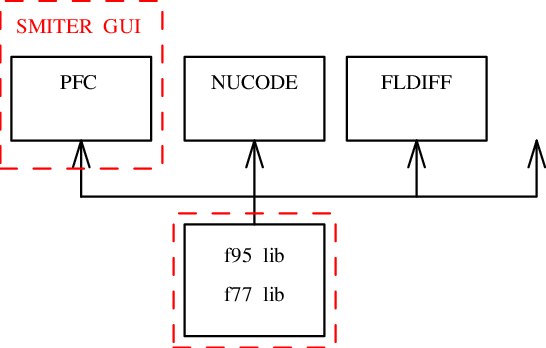
\includegraphics[width=0.7\textwidth]{../pics/layout}}
\caption{Library structure of the \F{SMARDDA} modules. The Fortran~95 (f95) library
contains modules used by one or more of application codes \F{SMARDDA-PFC},
\F{SMARDDA-NUCODE}, etc. (The parts of the software in red boxes form the kernel
of the ITER IMAS code~SMITER.)\label{fig:layout}}
\end{figure}

